\documentclass[a4paper,11pt,twoside]{article}
\usepackage[utf8]{inputenc}	% Text coding
\usepackage[T1]{fontenc}
\usepackage{lmodern}
\usepackage[czech]{babel}
\usepackage{epsfig}
\usepackage{amsfonts,amsmath,amssymb}
\usepackage{graphicx}
\usepackage[unicode]{hyperref}
\usepackage{indentfirst}
\usepackage{fancyhdr}
\usepackage{xifthen}
\usepackage{amsthm,thmtools}
\usepackage{bold-extra}
\usepackage[dvipsnames]{xcolor}
\usepackage[subrefformat=simple,labelformat=simple]{subcaption} % Instead of subfigure
\usepackage{listings}
\usepackage{comment}
\usepackage{titlesec}
\usepackage{underscore}
\usepackage{makecell}       % Šířky čar v tabulkách

% Page size
\addtolength{\topmargin}{-1.5cm} %\addtolength{\textheight}{-10cm}
\addtolength{\textwidth}{4cm} \addtolength{\textheight}{4cm} % Width and height of the text
\addtolength{\voffset}{-0.5cm} % Top margin
\addtolength{\hoffset}{-2cm}
\setlength{\headheight}{15pt}

\DeclareMathOperator{\e}{e}

\def\vector#1{\boldsymbol{#1}}								% Vector
\renewcommand{\d}{\mathrm{d}}
\newcommand{\derivative}[3][]{\ifthenelse{\isempty{#1}}	    % Normal derivative
	{\frac{\d{#2}}{\d{#3}}}
	{\frac{\d^{#1}{#2}}{\d{#3}^{#1}}}
}
\newcommand{\im}{\mathrm{i}}

\def\makematrix#1{\begin{pmatrix}#1\end{pmatrix}}       % Matrix
\def\abs#1{\left|#1\right|}
\def\probability#1{\mathrm{Pr}\left[#1\right]}
\def\expectation#1{\mathrm{E}\left[#1\right]}
\def\dispersion#1{\sigma_{#1}^{2}}

\def\code#1{\textnormal{\texttt{#1}}}
\def\file#1{\textnormal{\textbf{\texttt{#1}}}}
\def\ghfile#1#2{\textnormal{\textbf{\texttt{\href{https://github.com/PavelStransky/PCInPhysics2021/blob/main/#1#2}{#2}}}}}

\def\abbreviation#1{\textnormal{\textsc{#1}}}

\begin{document}

\section*{Zápočtová práce 1.6.2021}
\subsection*{Monte-Carlo simulace Isingova modelu}
\subsubsection*{Isingův model}
Isingův model je jednoduchý model magnetických vlastností pevné látky. 
Model spočívá v sadě $n$ \uv{spinů} (magnetických dipólů) $S_{j}$ uspořádaných na pravidelné mříži, přičemž interagují vždy pouze sousední spiny.
Podle počtu a uspořádání interakcí se odlišují různé typy a dimenzionality mříží: spiny na řetízku (1D), čtvercová nebo šesterečná mříž (2D), kubická mříž (3D), atd.
Každý spin $S_{j}$ může mít pouze jednu ze dvou hodnot: $+1$ nebo $-1$ (spin míří nahoru nebo dolů).

Energie systému (Hamiltonián) je dána vztahem
\begin{equation}\label{eq:Hamiltonian}
	E=H=-J\sum_{\text{sousedi }\langle jk\rangle}S_{j}S_{k},
\end{equation}
kde $J>0$ je konstanta udávající sílu interakce.
Znaménko $-$ zaručuje, že preferované uspořádání spinů při nulové teplotě je paralelní a odpovídá feromagnetické chování.

Střední magnetizace je 
\begin{equation}\label{eq:Magnetisation}
	M=\langle S_{j}\rangle=\frac{1}{n}\sum_{j=1}^{n}S_{j}.
\end{equation}

Termální fluktuace paralelní uspořádání spinů rozbíjí.
Při nekonečné velikosti mříže $n\rightarrow\infty$ vykazuje model termodynamický fázový přechod mezi feromagnetickou fází s $\abs{M}>0$ za teplot $T<T_{c}$ a paramagnetickou fází s $\abs{M}=0$ za teplot $T>T_{c}$, kde  $T_{c}$ je teplota fázového přechodu (kritická teplota, Curieova teplota).
Numericky lze fázový přechod pozorovat i pro konečnou velikost mříže.

\begin{figure}[!htbp]
	\centering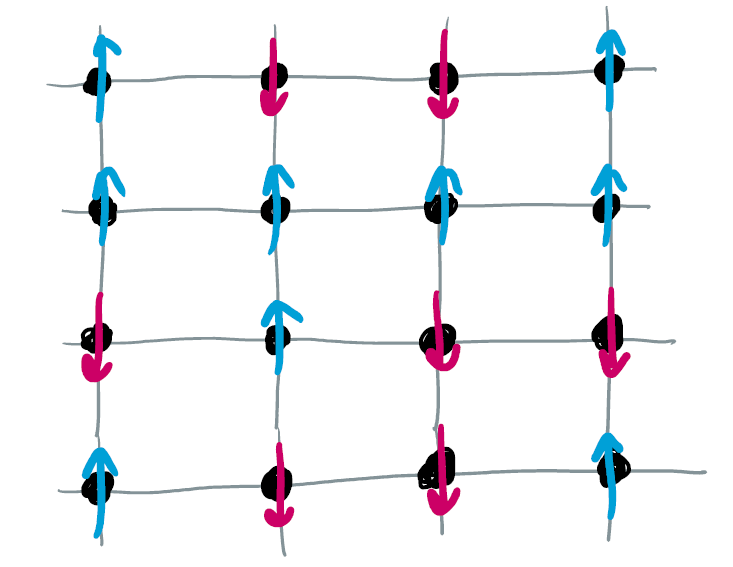
\includegraphics[width=0.495\linewidth]{Ising.png}
	\caption{
		\protect\small
		Isingův model na čtvercové 2D mříži.
		Černé puntíky: jednotlivé spiny.
		Modrá šipka nahoru: $S_{j}=+1$.
		Červená šipka dolů: $S_{j}=-1$.
		Šedé čáry: interakce.
		Zobrazená mříž odpovídá $N=4$ (rozměr mříže), $n=16$ (počet spinů v mříži).
	}	
	\label{fig:2DIsing}
\end{figure}

\subsubsection*{Metropolisův algoritmus}
Chování Isingova modelu za konečné teploty se simuluje \emph{Metropolisovým algoritmem}, který spočívá následujících krocích:
\begin{enumerate}
	\item Máme $n$ spinů $S_{j}$ rozmístěných na mříži.
	\item Měníme postupně stav (znaménko) každého spinu.
		Označme energii před změnou $E_{\mathrm{před}}$, energii po změně $E_{\mathrm{po}}$, rozdíl energií $\Delta E\equiv E_{\mathrm{před}}-E_{\mathrm{po}}$.
		Podud $\Delta E<0$, změnu přijmeme.
		Pokud $\Delta E>0$, změnu přijmeme s pravděpodobností
		\begin{equation}
			p=\e^{-\frac{\Delta E}{k_{B} T}},
		\end{equation}
		kde $k_{B}$ je Boltzmannova konstanta.
	\item Získáme nový stav mříže a výpočet opakujeme.
\end{enumerate}

Po spuštění Metropolisova algoritmu na náhodně nagenerovanou mříž trvá nějakou dobu, než se teplota mříže ustálí na požadované teplotě $T$.
Tento jev se nazývá \emph{relaxace}.
Nás bude zajímat chování systému v \emph{rovnovážném stavu}, tj. po relaxaci.

\subsubsection*{Úloha}
Uvažujte Isingův systém na dvourozměrné čtvercové mříži velikosti $N\times N$ (každý spin interaguje se čtyřmi sousedy, viz obrázek~\ref{fig:2DIsing}, celkový počet spinů je $n=N^2$) za konečné teploty $T$.

\begin{enumerate}
    \item \emph{(1 bod)} Zvolte vhodnou realizaci Isingovy čtvercové 2D mříže a napište funkci, která nageneruje náhodně její počáteční konfiguraci.
    
    \item \emph{(2 body)} Napište funkci, která spočítá energii Isingovy čtvercové mříže podle vzorce~\eqref{eq:Hamiltonian}.
		Předpokládejte cyklické okrajové podmínky.

    \item \emph{(1 bod)} Napište funkci, která spočítá střední magnetizaci Isingovy čtvercové mříže podle vzorce~\eqref{eq:Magnetisation}.
    
    \item \emph{(2 body)} Naprogramujte jeden krok Metropolisova algoritmu.
    
    \item \emph{(2 body)} Vytvořte funkci, která provede následující posloupnost výpočtů pro teplotu $T$:
    \begin{itemize}
		\item {\bf Inicializace}: Nageneruje náhodnou mříž (viz bod 1).
		\item {\bf Relaxace}: Pro mříž provede $r$ kroků Metropolisova algoritmu (viz bod 4).
		\item {\bf Výpočet magnetizace a energie}: Po relaxaci provede $m$ kroků Metropolisova algoritmu.
			Po každém kroku spočítá magnetizaci $M_k$ podle~\eqref{eq:Magnetisation} a energii $E_k$ podle~\eqref{eq:Hamiltonian}.
		\item {\bf Výsledek}: Funkce vrátí průměrnou hodnotu 
		\begin{equation}
			M=\frac{1}{m}\sum_{k=1}^{m}M_{k},\qquad E=\frac{1}{m}\sum_{k=1}^{m}E_{k}.
		\end{equation}
	\end{itemize}
	
	\item \emph{(2 body)} Využijte funkci z bodu 5 a nakreslete \emph{bodové} grafy funkcí $M=M(T)$, $E=E(T)$ pro $T\in\langle 0;4\rangle$.
		Zvolte dostatečné množství teplot (doporučuji 100 hodnot).
		Z grafů odhadněte Curieovu teplotu $T_{c}$.

\end{enumerate}

Program odlaďte pro mříž velikosti $N=10$.

Při výpočtech uvažujte $J=1$, $k_{B}=1$, $r=50$, $m=50$.

\end{document}